
\documentclass[a4paper,12pt]{article}
%%%%%%%%%%%%%%%%%%%%%%%%%%%%%%%%%%%%%%%%%%%%%%%%%%%%%%%%%%%%%%%%%%%%%%%%%%%%%%%%%%%%%%%%%%%%%%%%%%%%%%%%%%%%%%%%%%%%%%%%%%%%%%%%%%%%%%%%%%%%%%%%%%%%%%%%%%%%%%%%%%%%%%%%%%%%%%%%%%%%%%%%%%%%%%%%%%%%%%%%%%%%%%%%%%%%%%%%%%%%%%%%%%%%%%%%%%%%%%%%%%%%%%%%%%%%
\usepackage{eurosym}
\usepackage{vmargin}
\usepackage{amsmath}
\usepackage{graphics}
\usepackage{epsfig}
\usepackage{subfigure}
\usepackage{fancyhdr}
%\usepackage{listings}
\usepackage{framed}
\usepackage{graphicx}

\setcounter{MaxMatrixCols}{10}
%TCIDATA{OutputFilter=LATEX.DLL}
%TCIDATA{Version=5.00.0.2570}
%TCIDATA{<META NAME="SaveForMode" CONTENT="1">}
%TCIDATA{LastRevised=Wednesday, February 23, 2011 13:24:34}
%TCIDATA{<META NAME="GraphicsSave" CONTENT="32">}
%TCIDATA{Language=American English}

\pagestyle{fancy}
\setmarginsrb{20mm}{0mm}{20mm}{25mm}{12mm}{11mm}{0mm}{11mm}
\lhead{MA4128} \rhead{Mr. Kevin O'Brien}
\chead{Advanced Data Modelling}
%\input{tcilatex}


% http://www.norusis.com/pdf/SPC_v13.pdf
\begin{document}
\section{Clustering Linkage Methods}
\newpage

%----------------------------------------------------------%
% http://www2.statistics.com/resources/glossary/h/hclusteran.php

% http://mlsc.lboro.ac.uk/resources/statistics/Clusteranalysis.pdf

\section{Cluster Methods}
Having selected how we will measure distance, we must now choose the clustering algorithm, i.e. the rules that govern between which points distances are measured to determine cluster membership. There are many methods available, the criteria used differ and hence
different classifications may be obtained for the same data. This is important since it tells us that, although cluster analysis may provide an objective method for the clustering of cases, there can be subjectivity in the choice of method. 

The linkage distances are calculated by SPSS. The goal of the clustering algorithm is to join objects together into successively larger clusters, using some measure of similarity or distance. SPSS provides seven clustering algorithms, the most commonly used one being  \textbf{\textit{Ward's method}}.

SPSS provides several alternative methods for determining a summary measure of distance when a cluster has multiple cases in the cluster.  The SPSS options for the clustering method are Between-groups linkage, Within-groups linkage, Nearest neighbor, Furthest neighbor, Centroid clustering, Median clustering, and Ward's method.

\begin{itemize}
	\item For the \textbf{nearest neighbor} or \textbf{single linkage} method, the dissimilarity between cluster A and cluster B is represented by the minimum of all possible distances between the cases in cluster A and the cases in cluster B.
	
	\item For the \textbf{furthest neighbor} or \textbf{complete linkage} method, the dissimilarity between cluster A and cluster B is represented by the maximum of all possible distances between the cases in cluster A and the cases in cluster B.
	
	\item For the \textbf{between-groups linkage} or average linkage method, the dissimilarity between cluster A and cluster B is represented by the average of all the possible distances between the cases in cluster A and the cases in cluster B.
	
	\item For the \textbf{within-groups linkage} method, the dissimilarity between cluster A and cluster B is represented by the average of all the possible distances between the cases within a single new cluster determined by combining cluster A and cluster B.
	
	\item  
	For the \textbf{centroid clustering} method, the dissimilarity between cluster A and cluster B is represented by the distance between the centroid for the cases in cluster A and the centroid for the cases in cluster B.  Note that this distance is not mathematically equivalent to the average of the distances used in the average linkage method.  Also note the SPSS warning below about using squared Euclidean distance rather than Euclidean distance for this procedure.
	
	\begin{framed}
		The squared Euclidean measure should be used when the CENTROID, MEDIAN, or WARD cluster method is requested.
	\end{framed}
	
	\item For \textbf{Ward’s method}, the dissimilarity between cluster A and cluster B is represented by the “loss of information” from joining the two clusters with this loss of information being measured by the increase in error sum of squares.  For a cluster the sum of squares is the sum of squared deviations of each case from the centroid for the cluster.  The error sum of squares is the total of these for all clusters.  When selecting clusters to join, the two clusters among all possible combinations that have the minimum increase in error sum of squares are selected.  See the note above about using squared Euclidean distance rather than Euclidean distance for this method.
	
	\item 
	For the \textbf{median clustering} method, the dissimilarity between cluster A and cluster B is represented by the distance between the SPSS determined median for the cases in cluster A and the median for the cases in cluster B.  See the message in the note above about using squared Euclidean distance rather than Euclidean distance for this method.
	
\end{itemize}


\subsection{Nearest neighbour method} 
(\textit{Also known as the single linkage method}).\\
In this method the distance between two clusters is defined to be the distance between
the two closest members, or neighbours. This method is relatively simple but is often
criticised because it doesn’t take account of cluster structure and can result in a problem
called chaining whereby clusters end up being long and straggly. However, it is better
than the other methods when the natural clusters are not spherical or elliptical in shape.

\subsection{Furthest neighbour method}
(\textit{Also known as the complete linkage method}).\\
In this case the distance between two clusters is defined to be the maximum distance
between members  i.e. the distance between the two subjects that are furthest apart.
This method tends to produce compact clusters of similar size but, as for the nearest
neighbour method, does not take account of cluster structure. It is also quite sensitive
to outliers.

\subsection{Average (between groups) linkage method }
(\textit{sometimes referred to as UPGMA}).\\
The distance between two clusters is calculated as the average distance between all pairs
of subjects in the two clusters. This is considered to be a fairly robust method.

\subsection{Centroid method}
Here the centroid (mean value for each variable) of each cluster is calculated and the
distance between centroids is used. Clusters whose centroids are closest together are
merged. This method is also fairly robust.

\subsection{Ward’s method}
In this method all possible pairs of clusters are combined and the sum of the squared
distances within each cluster is calculated. This is then summed over all clusters. The
combination that gives the lowest sum of squares is chosen. This method tends to
produce clusters of approximately equal size, which is not always desirable. It is also
quite sensitive to outliers. Despite this, it is one of the most popular methods, along
with the average linkage method.

%\subsection{Ward's Method}
%This method is distinct from other methods because it uses an \textbf{\textit{analysis of variance}} approach to evaluate the distances between clusters. In general, this method is very efficient.
%
%Cluster membership is assessed by calculating the total sum of squared deviations from the mean of a cluster. The criterion for fusion is that it should produce the smallest possible increase
%in the error sum of squares.
%
%
%
%\subsection{Ward's Linkage}
%
%Ward's linkage is a method for hierarchical cluster analysis . The idea has much in common with analysis of variance (ANOVA). The linkage function specifying the distance between two clusters is computed as the increase in the "error sum of squares" (ESS) after fusing two clusters into a single cluster. Ward's Method seeks to choose the successive clustering steps so as to minimize the increase in ESS at each step.



\subsection{Linkage methods}
\begin{itemize}
	\item  Single linkage (minimum distance)
	\item  Complete linkage (maximum distance)
	\item  Average linkage
\end{itemize}

%http://www.rdg.ac.uk/~aes02mm/supermarket.sav

\subsubsection{Ward's method}
\begin{itemize}
	\item  Compute sum of squared distances within clusters
	\item  Aggregate clusters with the minimum increase in the
	overall sum of squares
\end{itemize}
\subsubsection{Centroid method}
The distance between two clusters is defined as the
difference between the centroids (cluster averages)

\begin{itemize}

\item A commonly used approach in hierarchical clustering is \textbf{\textit{Ward’s linkage method}}.
This approach does not combine the two most similar objects successively. Instead,
those objects whose merger increases the overall within-cluster variance to the
smallest possible degree, are combined. If you expect somewhat equally sized
clusters and the data set does not include outliers, you should always use Ward’s
method.

We will use the Ward's linkage method for laboratory exercises.


\item Other most popular
agglomerative clustering procedures include the following:
\begin{description}
	\item[Single linkage (nearest neighbor)]: The distance between two clusters corresponds
	to the shortest distance between any two members in the two clusters.
	\begin{figure}[h!]
		\begin{center}
			% Requires \usepackage{graphicx}
			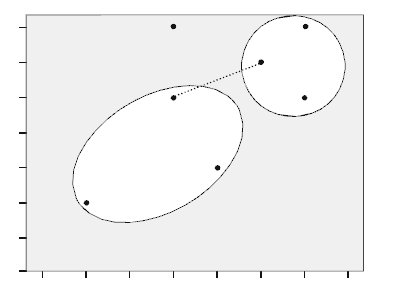
\includegraphics[scale=0.4]{images/Link1.jpg}\\
		\end{center}
	\end{figure}
	\item[Complete linkage (furthest neighbor)]: The oppositional approach to single
	linkage assumes that the distance between two clusters is based on the longest
	distance between any two members in the two clusters.
	\begin{figure}[h!]
		\begin{center}
			% Requires \usepackage{graphicx}
			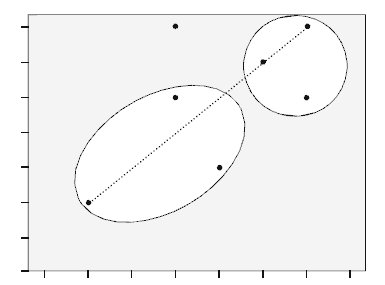
\includegraphics[scale=0.4]{images/Link2.jpg}\\
		\end{center}
	\end{figure}
	\item[Average linkage] : The distance between two clusters is defined as the average
	distance between all pairs of the two clusters’ members.
	\begin{figure}[h!]
		\begin{center}
			% Requires \usepackage{graphicx}
			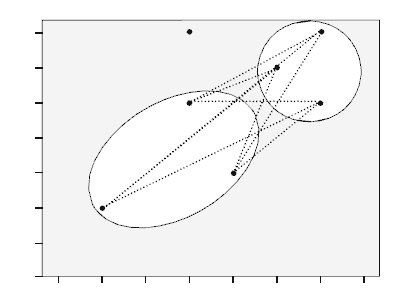
\includegraphics[scale=0.4]{images/Link3.jpg}\\
		\end{center}
	\end{figure}
	\newpage
	\item[Centroid] : In this approach, the geometric center (centroid) of each cluster is
	computed first. The distance between the two clusters equals the distance between
	the two centroids.
	\begin{figure}[h!]
		\begin{center}
			% Requires \usepackage{graphicx}
			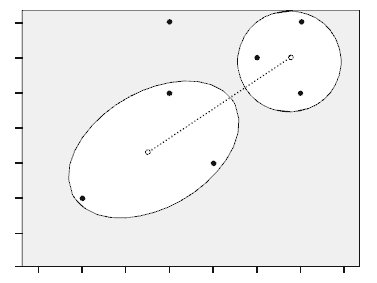
\includegraphics[scale=0.4]{images/Link4.jpg}\\
		\end{center}
	\end{figure}
\end{description}
Each of these linkage algorithms can yield totally different results when used on the same data set, as each has its specific properties. As the single linkage algorithm is based on minimum distances, it tends to form one large cluster with the other clusters containing only one or few objects each. We can make use of this \textbf{\textit{chaining effect}} to detect outliers, as these will be merged with the remaining objects – usually at very large distances – in the last steps of the analysis. Generally, single linkage is considered the most versatile algorithm.

Conversely, the complete linkage method is strongly affected by outliers, as it is based on maximum distances. Clusters produced by this method are likely to be rather compact and tightly clustered. The average linkage and centroid algorithms tend to produce clusters with rather low within-cluster variance and similar sizes.
However, both procedures are affected by outliers, though not as much as complete linkage.

An understanding of linkage method's other than than Ward method will be expected in the end of year examination.

\item A common way to visualize the cluster analysis’s progress is by drawing a
dendrogram, which displays the distance level at which there was a combination
of objects and clusters.
Here is an example of a dendrogram (which corresponds to the example in the next section of material.


\begin{figure}[h!]
	\begin{center}
		% Requires \usepackage{graphicx}
		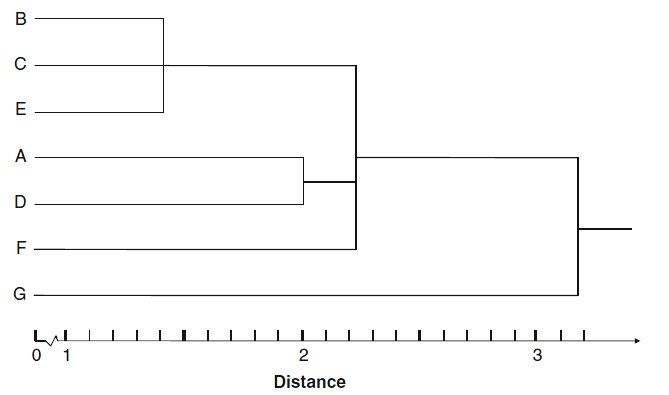
\includegraphics[scale=0.6]{images/Dendrogram.jpg}\\
	\end{center}
\end{figure}

\item An important question is how to decide on the number of
clusters to retain from the data. Unfortunately, hierarchical methods provide only
very limited guidance for making this decision. The only meaningful indicator
relates to the distances at which the objects are combined. Similar to factor
analysis’s scree plot, we can seek a solution in which an additional combination
of clusters or objects would occur at a greatly increased distance. This raises the
issue of what a great distance is, of course. For this purpose, we can make use of the dendrogram.

\item In constructing the dendrogram, SPSS rescales the distances to a range of 0–25; that is, the last merging step to a one-cluster solution takes place at a
(rescaled) distance of 25. The rescaling often lengthens the merging steps, thus
making breaks occurring at a greatly increased distance level more obvious. Despite this, this distance-based decision rule does not work very well in all
cases.

It is often difficult to identify where the break actually occurs. This is also
the case in our example above. By looking at the dendrogram, we could justify
a two-cluster solution ([A,B,C,D,E,F] and [G]), as well as a five-cluster solution
([B,C,E], [A], [D], [F], [G]).


\item 
The clustering algorithm is based on a distance measure that gives the best results if all variables are independent, continuous variables have a normal distribution (or categorical variables have a multinomial distribution). This is seldom the case in practice, but the algorithm is thought to behave reasonably well when the assumptions are not met.

\item 
Because cluster analysis does not involve hypothesis testing and calculation of observed significance levels, other than for descriptive follow-up, it's perfectly acceptable to cluster data that may not meet the assumptions for best performance.
\item 
The final outcome may depend on the order of the cases in the file. To minimize the effect, arrange the cases in random order. Sort them by the last digit of their ID numbers or something similar.
\end{itemize}
\newpage


%----------------------------------------------------------%
% http://www2.statistics.com/resources/glossary/h/hclusteran.php

% http://mlsc.lboro.ac.uk/resources/statistics/Clusteranalysis.pdf


%\subsection{Ward's Method}
%This method is distinct from other methods because it uses an \textbf{\textit{analysis of variance}} approach to evaluate the distances between clusters. In general, this method is very efficient.
%
%Cluster membership is assessed by calculating the total sum of squared deviations from the mean of a cluster. The criterion for fusion is that it should produce the smallest possible increase
%in the error sum of squares.
%
%
%
%\subsection{Ward's Linkage}
%
%Ward's linkage is a method for hierarchical cluster analysis . The idea has much in common with analysis of variance (ANOVA). The linkage function specifying the distance between two clusters is computed as the increase in the "error sum of squares" (ESS) after fusing two clusters into a single cluster. Ward's Method seeks to choose the successive clustering steps so as to minimize the increase in ESS at each step.

\end{document}
